\documentclass[12pt]{article}
\usepackage{amsmath}
\usepackage{array}
% \usepackage{gensymb}
\usepackage{geometry}
\usepackage{graphicx}
\usepackage{pgfplots}
\usepackage{siunitx}
\usepackage{wrapfig}

\title{Homework \#8}
\author{Donald Aingworth IV}
\date{October 16, 2024}

\pgfplotsset{width=8cm,compat=1.9}
\usepgfplotslibrary{external}
% \tikzexternalize

\begin{document}

\DeclareSIUnit{\mile}{mi}
\DeclareSIUnit{\gal}{gal}
\DeclareSIUnit{\foot}{ft}
\DeclareSIUnit{\h}{h}

% \maketitle

% \pagebreak
\section*{Problem 1}
A spring gun with k = 90.0 N/m is compressed by 5 cm. What is the exit speed of a 2.10-g projectile?

\subsection*{Solution}

\begin{align*}
    W   &= \int_{min}^{max} F(x)\ dx = \int_{-0.05}^{0} -kx\ dx = \left(-\frac{1}{2}kx^2\right)\vert_{-0.05}^{0} \\
        &= \frac{1}{2}k*0.05^2 = 45\unit{\newton/\meter} * 0.0025\unit{\meter^2} = 0.1 \unit{\joule}\\
    W   &=  \Delta K = K_f - K_i
\end{align*}
Since the spring on the block is unmoving at the start, then $v_i = 0$, so $K_i = \frac{1}{2}mv_i^2$ is also equal to zero. From there, we can determine the final kinetic energy and determine the velocity at the end.

\begin{align*}
    K_f &= W = 0.1\unit{\joule} = \frac{1}{2}mv_f^2\\
    \frac{2K_f}{m} &= v_f^2\\
    v_f &= \sqrt{\frac{2K_f}{m}} 
        = \sqrt{\frac{2*0.1\unit{\joule}}{0.0021\unit{\kilo\gram}}}
        = \sqrt{\frac{2*1000}{21}}\\
        &= \boxed{\frac{20\sqrt{105}}{21} \unit{\meter/\second} \approx 9.759 \unit{\meter/\second}}
\end{align*}

\pagebreak
\section*{Problem 2}
(a) The United States, with a population of $2.2 \times 10^8$ people, consumes $5 \times 10^{19}$ J per year. What is the per capita consumption in watts? (b) The sun's radiation provides the earth with 1000 \unit{\watt/\meter^2}. Assuming solar energy can be converted to electrical energy with a 20\% efficiency, how much area is needed to serve the energy needs of each U.S. citizen?

\subsection*{Solution}
\subsubsection*{Section (a)}
The power is determined by the work ($W$) divided by the time, with a watt being a joule divided by a second. The per capita value is determined by division by the number of humans ($c$). Assuming a year of 365 days, we can calculate the number of seconds per year ($t$) first.
\begin{align*}
    t   &=  1 \text{ years} * \frac{365\text{ days}}{1\text{ years}} 
                            * \frac{24\text{ hours}}{1\text{ days}}
                            * \frac{3600\unit{\second}}{1\text{ hours}}
        =   31536 \times 10^3 \unit{\second}\\
    P   &=  \frac{W}{t}
        =   \frac{5 \times 10^{19} \unit{\joule}}{(31536 \times 10^3 \unit{\second})}
        =   \frac{5 \times 10^{16}}{31536} \unit{\watt}\\
        &=  1.58549 \times 10^{12}\ \unit{\watt}\\
    P_{per\ captia}  &=  \frac{1.58549 \times 10^{12}}{2.2 \times 10^8} \unit{\watt}\\
        &=  \boxed{ 7206.77 \unit{\watt} }
\end{align*}

\subsubsection*{Section (b)}
Since there is only a 20\% efficiency, the usable numbers of watts per square meter would be $ Wa = 1000\ \unit{\watt/\meter^2}*\frac{20}{100} = 200\ \unit{\watt/\meter^2} $. We can divide the total power necessary per citizen (which we calculated in part (a)) to get the area necessary.
\begin{align*}
    A   &= \frac{P}{Wa}
        = \frac{ 7206.77 \unit{\watt} }{ 200\ \unit{\watt/\meter^2} }
        = \boxed{36.03 \unit{\meter^2}}
\end{align*}

\pagebreak
\section*{Problem 3}
A 0.595-kg object is released from a height of 3.60 m and lands on the ground. Find: (a) the work done by gravity; (b) the change in kinetic energy of the ball; (c) the speed just before it lands using energy methods. Ignore air resistance.

\subsection*{Solution}


\pagebreak
\section*{Problem 4}
\begin{wrapfigure}{r}{0.35\textwidth}
    \vspace{-30pt}
    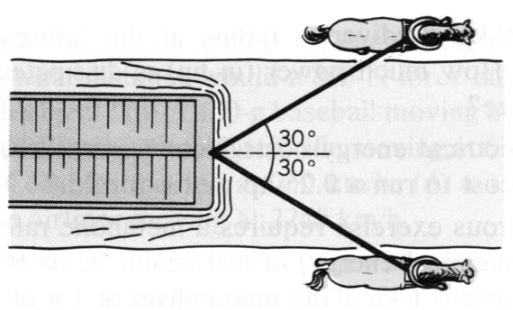
\includegraphics[width=0.35\textwidth]{graph_4.png} 
    % \label{fig:wrapfig}
\end{wrapfigure}
Two horses pull a barge along a canal at a steady 5.00 km/h, as shown in the figure. The tension in each rope is 420 N and each is at 300 to the direction of motion. What is the horsepower provided by the horses?

\subsection*{Solution}


\pagebreak

\end{document}